\documentclass[a4paper, 12pt]{article}

\usepackage[T1]{fontenc}
\usepackage[english]{babel}
\usepackage{hyperref}
\usepackage{url}
\usepackage{amsmath}
\usepackage{amsfonts}
\usepackage{framed}
\usepackage{graphicx}
%\usepackage{subfigure}
\usepackage{subfig}
%\graphicspath{{s/}}

\begin{document}


\begin{titlepage}
\begin{center}

{\huge \bfseries
Parallel Optimization Workbench (POW)\\
- User Manual -\\}
\ \\
\ \\
\vspace{3cm}
% split the page into two columns
% left column
%\begin{minipage}{0.4\textwidth}
%\begin{flushleft} \large
%Matteo T. Degiacomi, Matteo Dal Peraro \\
%\end{flushleft}
%\end{minipage}

% ensure vertical alignment with LHS
\footnotesize{\ }
\vfill % fill vertical space
%
% Bottom of the page
% \today is the compilation date
{\large Laboratory For Biomolecular Modeling, Institute of Bioengineering, School of Life Sciences, Ecole Polytechnique F\'ed\'erale de Lausanne - EPFL, Lausanne, Switzerland}
%
\end{center}
\end{titlepage}


\pagebreak

\pagestyle{plain}
\parindent=0in

\tableofcontents

\pagebreak


\section{Requirements}

POW requires the following python (>=2.5) packages to be installed:
\begin{itemize}
\item \texttt{numpy}
\item \texttt{mpi4py}
\end{itemize}

The execution of parallel calculation will also require the installation of OpenMPI. Additonal packages may be required by specific POW modules:

\begin{itemize}
\item \texttt{scipy}, used by the modules \texttt{DockDimer} and \texttt{DockSymmCircle}
\item \texttt{MDAnalysis}, used by the modules \texttt{DockDimer} and \texttt{DockSymmCircle}
\item \texttt{wxpython}, required when running the GUI of the \texttt{Function} module 
\end{itemize}


\section{Architecture}

POW is a framework allowing the resolution of virtually any optimization problem via the addition of a specific module. This object oriented code is developed in Python, and supports parellel computation by exploiting MPI libraries. The architecture of our framework is represented in Figure \ref{architecture}. Every box corresponds to a specific class. Classes highlighted in blue are common to any optimization problem, and can be considered as a black box by the user. Classes in the yellow area change depending on the problem being solved. We will call \emph{module} a file containing an implementation for these classes aiming at solving a specific problem. In order to use POW, a user has to provide two information: the module name, and a parameterization file.\\  

\begin{figure}[htp!]
\centering
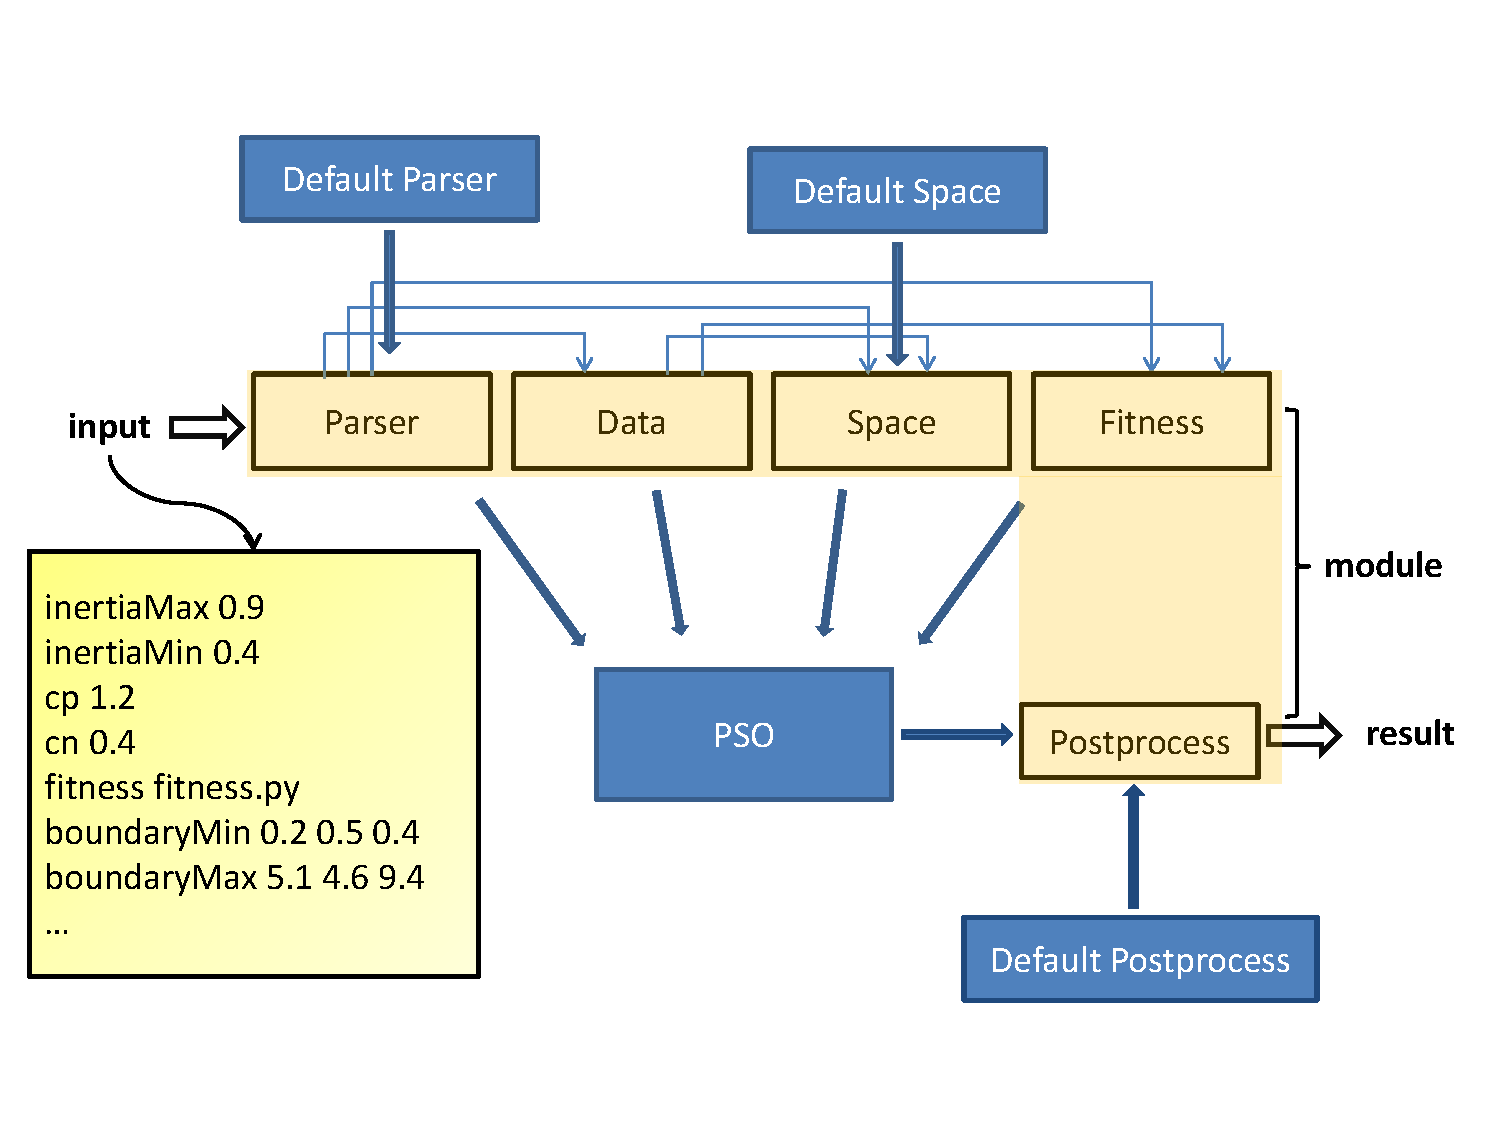
\includegraphics[scale=0.55]{PSO-architecture.pdf}
\caption{\emph{Schematic of the Optimizer architecture. Every box represent a class. Classes highlighted in blue are common to any optimization problem, and can be considered as a black box for by the user. Classes in the yellow area change depending on the problem being solved. We call a module a file containing a definition for these classes aimed at solving a specific problem. Input is provided as a text file containing keywords with associated values.}}
\label{architecture}
\end{figure}

The parameterization file contains a set of keywords associated to one or more values. Some keywords are standard for any optimization problem, whereas others are problem specific. The classes \texttt{DefaultParser} (for standard keywords) and \texttt{Parser} (for custom ones) are in charge of reading the input file.\\
Once the parameters are parsed POW loads, if needed, specific data structures required by the user. This operation is performed by the class \texttt{Data}. Since this class is part of a module, depending on how this class is implemented, any data structure can be manipulated.\\
Subsequently, POW defines the problem's search space. Every dimension of the search space is defined by upper and lower boundaries, as well as by specific boundary conditions. Creation of the search space is problem specific, and is managed by the \texttt{Space} class. Converseley, management of boundary conditions is the same for any optimization problem, and is implemented in the \texttt{DefaultSpace} class.\\
The class \texttt{PSO} implements POW's optimizer. The optimizer consists of a variation of a Particle Swarm Optimization algorithm, called PSO Kick and Reseed (PSO-KaR). The behavior of the optimizer is defined by an ensemble of parameters called \emph{inertia}, \emph{personal best} (\texttt{cp}), \emph{neighborhood best} (cn) and \emph{kar threshold} (\texttt{kar\_threshold}). Default values for these parameters are set, the user is however free to set them at will using specific keywords in the parameterization file (see section Standard Keywords).\\ 
Along the optimization run, every measure performed by every particule is stored in a log file. In order to extract useful information, postprocessing this log file is necessary. The class \texttt{Postprocess} is in charge of this. Useful functions the user might need, such as the selection of measures below a given threshold, are preimplemented in the \texttt{DefaultPostprocess} class.\\

POW has been concieved so that the creation of a new module (i.e. a specific implementation of the \texttt{Parser}, \texttt{Data}, \texttt{Space}, \texttt{Fitness} and \texttt{Postprocess} classes) is trivial even for a user unaware of its internal architecture. The following modules are already available:

\begin{itemize}
\item DockDimer: dock two proteins into an heterodimer
\item DockSymmCircle: rigid/flexible assembly of n monomers according to a circular symmetry, possibly in presence of a receptor
\item Function: generic function optimization
\end{itemize}

In the next sections these modules will be described.


\section{Provided Files}

The compressed folder \emph{POW.tar.gz} containing all the needed files is downloadable at \href{http://lbm.epfl.ch/resources}{lbm.epfl.ch/resources}. This file unpacks in a folder called POW, which can be placed anywhere in your computer. The folder contains the following files:
\begin{itemize}
\item \texttt{Assembly.py} : data structure for heterodimers assembly
\item \texttt{Default.py}: classes common to any POW implementation
\item \texttt{DockDimer.py}: dock two proteins
\item \texttt{DockSymmCircle.py}: rigid/flexible assembly of n monomers according to a circular symmetry, possibly around a given receptor
\item \texttt{Function.py}: generic function optimization
\item \texttt{flexibility.py}: functions for Principal Components Analysis
\item \texttt{parse.py}: performs just the postprocessing, without running PSO. This is useful when POW has been already run, and just alternate postprocessing options on the produced results have to be tried. Usage goes as follow:\\
\texttt{./parse.py module input\_file [logfile]}
\item \texttt{POW.py}: main executable
\item \texttt{Protein.py}: PDB parser
\item \texttt{PSO.py}: parallel implementation of Particle Swarm Optimization
\end{itemize}


\section{Launching}

POW is launched in the console by means of the following command:
\begin{verbatim}
mpiexec -n 4 $INSTALLATION_PATH/POW module input.dat
\end{verbatim}
It is advised to create an alias, in order to make POW execution easier. The following lines create a default call using 4 processors:
\begin{verbatim}
export NPROC=4
alias pow="mpiexec -n $NPROC $POW_DIR/POW.py"'
\end{verbatim}
An execution becomes now as simple as:
\begin{verbatim}
pow module input.dat
\end{verbatim}
This call will launch POW on 4 processors. A proper execution requires the user to provide two arguments to the call: the desired optimization module \texttt{module} and a parameterization file \texttt{input.dat}. The parameterization file describes with a series of keywords how POW should behave. The input file providing all the parametrisations for the search should be passed as parameter. The file is structured as a serie of keywords (one per line) having one or more corresponding values. Keywords are case sensitive, and their order is irrelevant. Some keywords are necessary for any kind of optimization procedure (see section \label{default}), whereas other are module specific (see sections dedicated to specific modules). The \# symbol can be used to comment out lines in parameterization file.


\section{Standard Keywords \label{default}}

The following keywords (implemented in \texttt{Default.py}) are typical to any optimization problem, and are therefore accessible by any module:

\subsection{Optimizer Behavior}

\begin{itemize}

\item steps $< number\ of\ steps\ to\ perform >$\\
\textbf{Acceptable values:} positive integer\\
\textbf{Default value:} 100\\
\textbf{Description:} The number of steps that will be computed in the \emph{PSO}.

\item particles $< number\ of\ particles >$\\
\textbf{Acceptable values:} positive integer\\
\textbf{Default value:} 40\\
\textbf{Description:} The number of particles that will be used in each step of the \emph{PSO}.

\item repeat $< number\ of\ repetition>$\\
\textbf{Acceptable values:} positive integer\\
\textbf{Default value:} 1\\
\textbf{Description:} Repeat can be used to lauch \emph{PSO} multiple, consecutive times. This is useful in order to enhance the sampling.

\item repulsion $< activate\ |\ desactivate >$\\
\textbf{Acceptable values:} on $|$ off\\
\textbf{Default value:} off\\
\textbf{Description:} When repulsion is activated, every good solution (solution smaller than \texttt{filter\_threshold}, particle velocity converging to zero) found by PSO will be flagged. Particles will be repelled by flagged regions with a $x^{-2}$ potential. When performing multiple PSO repetitions, flags are passed from one PSO run to the following one. This enhances PSO sampling, since regions where a minima has been already discovered are not oversampled. \emph{This option is currently experimental!}.

\item inertiaMax $< max\ inertia\ of\ particles >$\\
\textbf{Acceptable values:} float 0-1\\
\textbf{Default value:} 0.9\\
\textbf{Description:} It is the maximum inertia of particles. Between steps of the \emph{PSO} the inertia is decreased until \emph{inertiaMin}.

\item inertiaMin $< min\ inertia\ of\ particles >$\\
\textbf{Acceptable values:} float 0-1\\
\textbf{Default value:} 0.4\\
\textbf{Description:} It is the minimum inertia of particles. Between steps of the \emph{PSO} the inertia is decreased until \emph{inertiaMin}.

\item cp $< influence\ of\ local\ best\ solution >$ \\
\textbf{Acceptable values:} float\\
\textbf{Default value:} 1.2\\
\textbf{Description:} It is the influence on a particle of the best solution found by that particle. 

\item cn $< influence\ of\ global\ best\ solution >$\\
\textbf{Acceptable values:} float\\
\textbf{Default value:} 1.4\\
\textbf{Description:} It is the influence on a particle of the best position found by neighbors of that particle. 

\item kar\_threshold $< threshold\ for\ kar\ execution >$\\
\textbf{Acceptable values:} float > 0\\
\textbf{Default value:} 0.01\\
\textbf{Description:} When a particle is being slower than this threshold, the kick and reseed procedure (KaR) will be triggered. The particle will receive a random kick that will reaccelerate it. If, moreover, the particle's current fitness is smaller than filter\_threshold, it will be also reseeded in a random location. This avoids early convergence and forces the swarm to explore further the search space. Notice that setting kar\_threshold to 0 disables KaR.

\item neighborType $< type\ of\ neighbor>$\\
\textbf{Acceptable values:} indexed $|$ geographic\\
\textbf{Default value:} geographic\\
\textbf{Description:} NeighborType set the kind of neighborship between particles. In indexed neighborhood, particles are assigned an index, and particles having consecutive indexes are considered as neighbots. In geographic neighborhood, distance within particles in the search space is considered.

\item neighborSize $< number\ of\ neighbor>$\\
\textbf{Acceptable values:} positive integer\\
\textbf{Default value:} 1\\
\textbf{Description:} NeighborSize defines the amount of neighbors taken into account by every particle.
\end{itemize}

\subsection{Search Space definition}

\begin{itemize}

\item boundaryMin $< min\ boundary\ for\ each\ dimension >$\\
\textbf{Acceptable values:} list of lower boundary for each dimension, separated by spaces.\\
\textbf{Default value:} module dependent \\
\textbf{Description:} It is the minimum boundary for each dimension of the space. The first three values correspond to the rotations of the monomer on x, y and z axis respectively. The last one is the value specified by the \emph{radius} keyword. In case you did not use the \emph{radius} keyword, you MUST specify a minimum radius here.

\item boundaryMax $< max\ boundary\ for\ each\ dimension >$\\
\textbf{Acceptable values:} list of upper boundary for each dimension, separated by spaces.\\
\textbf{Default value:} module dependent\\
\textbf{Description:} It is the maximum boundary for each dimension of the space. The first three values correspond to the rotations of the monomer on x, y and z axis respectively. The last one is the value specified by the \emph{radius} keyword. In case you did not use the \emph{radius} keyword, you MUST specify a maximum radius here.

\item boundaryType $< type\ of\ the\ boundary >$\\
\textbf{Acceptable values:} 0 $|$ 1\\
\textbf{Default value:} module dependent\\
\textbf{Description:} For each dimension it is possible to define the boundary condition. \emph{0} and  \emph{1} stands for periodic and repulsive boundary conditions respectively.

%\item velocityMax $< max\ velocity\ of\ particles >$\\
%\textbf{Acceptable values:} list of maximum velocity in each dimension\\
%\textbf{Default value:} As default, this value is automatically calculated as boundaryMax - boundaryMin.\\
%\textbf{Description:} It is the maximum velocity for each dimension of the space. The first three values correspond to the rotations of the monomer on x, y and z axis respectively. The last one correspond to the radius of the multimer.

\end{itemize}

\subsection{Output options}

\begin{itemize}

\item filter\_threshold $< fitness\ value\ to\ accept >$\\ 
\textbf{Acceptable values:} float\\
\textbf{Default value:} 0\\
\textbf{Description:} An ensemble of solution is found, but just some of these will be good. This variable sets a threshold on the solutions fitness function.

\item output $< text\ file >$\\
\textbf{Acceptable values:} UNIX filename\\
\textbf{Description:} The text file will be used to store results.
 
\item restart\_freq $< restrart\ writing\ frequency >$\\
\textbf{Acceptable values:} int\\
\textbf{Default value:} round(steps/10)\\
\textbf{Description:} POW can automatically generate restart files saving the swarm state. These can be used to restart the optimization process after a crash. Setting this variable to $-1$ will disable restart writing.

\item save\_restart $< restart\ saving\ file\ name >$\\
\textbf{Acceptable values:} UNIX filename\\
\textbf{Default value:} swarm.restart\\
\textbf{Description:} Name of the restart file POW will automatically save at a frequency given by restat\_freq. The restart contains information about timestep, repetition, particles positions, velocities as well as position and value of their respective current best solution. During execution, both the most recent restart and an older copy of it are stored (default name \texttt{swarm.restart.old})
 
\item load\_restart $< restart\ loading\ file\ name >$\\
\textbf{Acceptable values:} UNIX filename\\
\textbf{Description:} By providing a restart file, the optimization process will restart from the last saved timestep and repetition. When restarting an optimization, the original input file should not be changed (the addition of load\_restart statement is sufficient). The previous log file will be backed up, and a new one will be generated. The new log file will contain all the data of previous logfile recordered until the restart point. If the old log file is not found, a new one is started.

\end{itemize}


\section{Function Module}

The \texttt{Function} module allows the minimization of any function not requiring manipulation of any data structure. The file containing the fitness function to be evaluated is passed to POW via the following keyword:

\begin{itemize}
\item fitness $< fitness\ extraction\ file >$\\
\textbf{Acceptable values:} UNIX filename\\
\textbf{Default value:} fit\_multimer\\
\textbf{Description:} This file contains the implementation for the Fitness class, and should have the following form:
\begin{verbatim}
class Fitness:
    def __init__(self,data,params):
        pass
    def evaluate(self, num, pos):
        #num: PSO particle index
        #pos: array of particle's position in search space 
        #compute fitness on the base of pos values
        return fitness
\end{verbatim}
\end{itemize}

The \texttt{Function} module can also be operated via a graphical interface invoked with the command \texttt{Function\_GUI.py} (see Figure \ref{psoGui}).
The interface allows the user to create, edit and save a POW input file, validate it, and launch a POW run on multiple processors.
Notice that the use of this graphical interface also requires the \texttt{wxPython} package to be installed.

\begin{figure}[htp!]
\centering
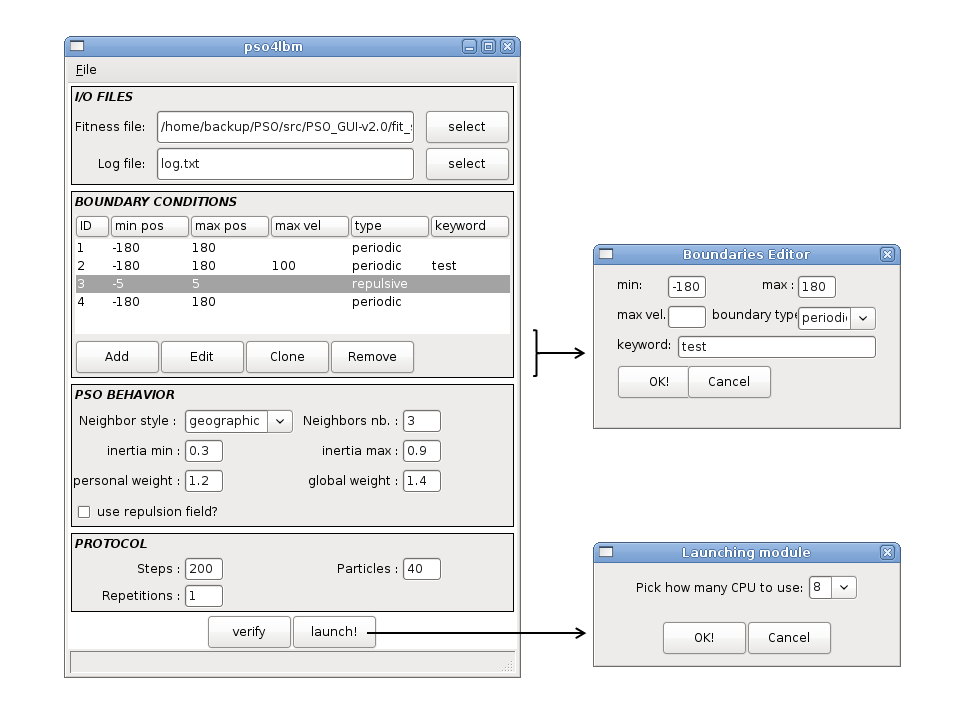
\includegraphics[scale=0.5]{powGui.png}
\caption{\emph{POW graphical interface for \texttt{Function} module} allowing the user to save, edit, validate and launch POW input files.}
\label{psoGui}
\end{figure}

\section{DockSymmCircle module}

\subsection{Overview}

With this POW module we aim at finding quickly a reasonable prediction for a multimeric structure arrangement on the basis of structural information about its subunits and experimental measures acting as search restraints. In a first step, an ensemble of monomer conformations is generated, typically from molecular dynamics simulations or structural biology experiments; this will be treated as a conformational database (see Material and Methods). The advantage of such an approach is that assembly prediction is performed using physically plausible structures.\\
Upon definition of a list of geometric restraints and a specific symmetry, a Particle Swarm Optimization (PSO) search subsequently tries to arrange the elements of the conformational database in a multimeric assembly so that all restraints are respected, and steric clashes avoided. Geometric restraints can be typically provided by low resolution electron density maps or experiments such as cross-linking disulfide scanning, mutagenesis or FRET. If necessary, POW can assemble a multimer on a given substrate. At PSO search completion, a large set of solutions having a good score is usually generated. A smaller set of representative solutions, typically less than ten, is returned by clustering the accepted solutions according to their respective Root Mean Square Deviation (RMSD).\\

At present, POW can predict hetero-dimers (when no symmetry is imposed, i.e. addressing general protein-protein interactions) or homo-multimers with or without a target substrate (if a circular symmetry is defined). This process is usually very fast (less than 5 minutes on an average workstation, using 4 processors), and can produce small ensemble of solutions being sufficiently good to generate biologically sound working hypotheses, and act as seeds for further optimization steps using more computationally expensive techniques.

\subsection{Implementation Details}

\subsubsection{Data Structures \label{symmdata}}

In order to manipulate protein structures, two classes are implemented: \texttt{Protein} and \texttt{Multimer}.\\

The \texttt{Protein} class allows to parse a PDB file, manipulate its coordinates, and extract the coordinates of specific atom selections. If (instead of a simple PDB file) an ensemble of structures is provided, POW will create a PDB called \texttt{protein.pdb} which will be parsed and subsequently used as an index. The ensemble of structures will be saved as a set of alternate coordinates. In detail, the following methods are implemented:

\begin{itemize}
\item \texttt{import\_pdb(pdb)}: parse a PDB file
\item \texttt{coords=get\_xyz()}: get cartesian coordinates of every atom. Returns a numpy $Nx3$ array, where $N$ is the number of atoms.
\item \texttt{set\_xyz(coords)}: set cartesian coordinates of every atom. \texttt{coords} must be a $Nx3$ array, where $N$ is the number of atoms.
\item \texttt{rotation(x,y,z)}: rotate the protein according to angles around the $x$,$y$ and $z$ axis.
\item \texttt{r=rgyr()}: compute gyration radius \texttt{r}
\item \texttt{c=center()} compute geometric center \texttt{c}
\item \texttt{coords=atomselect(chain,resid,atom)}: get cartesian coordinates of a subgroup of atoms selected by their chain name \texttt{chain}, residue id \texttt{resid} and atom name \texttt{atom}. Returns a numpy $Mx3$ array, where $M$ is the number of slected atoms. Chain, resid and atom can be also a wildcard symbol "*" (selecting all atoms). 
\item \texttt{write\_pdb(outname)}: save a new PDB file.
\end{itemize}

Note that, in order to speedup the calculation and simplify data storage, \texttt{Protein} stores a PDB as a numerical numpy array. Every chain name, atom name and residue name are converted into a numerical equivalent using a dictionnary.\\

The \texttt{Multimer} class is responsible of assemblying multimers on the base of an initially given \texttt{Protein} object. At the moment, this class can just produce multimers according to a circular symmetry. In detail, the following methods are implemented:

\begin{itemize}
\item \texttt{create\_multimer(degree, radius, pos)}: creates a circular multimer composed of \texttt{degree} monomers, having an internal radius equal to \texttt{radius} and having every monomer rotated according to \texttt{pos=[x,y,z]}. Notice that pos should be a numpy array. This is the first method to call after initialization. A list of \texttt{degree} length of numpy arrays containing a copy or \texttt{Protein} coordinates is created. Subsequently, every element in the list is individually manipulated to create a multimeric arrangement.
\item \texttt{multimer\_to\_origin()}: move the whole complex to the origin.
\item \texttt{z\_to\_origin()}: move the complex to place its center of geometry at $z=0$.
\item \texttt{cords=atomselect(unit,chain,resid,atom)}: get cartesian coordinates of a subgroup of atoms selected by their unit id \texttt{unit} (numbering of individual monomers counted clockwise), chain name \texttt{chain}, residue id \texttt{resid} and atom name \texttt{atom}.
\item \texttt{w=get\_width()}: get multimer width \texttt{w}.
\item \texttt{h=get\_height()}: get multimer height \texttt{h}.
\item \texttt{d=distance(select1, select2)}: compute the minimal euclidean distance between two sets of points \texttt{select1} and \texttt{select2}.
\item \texttt{coords=get\_multimer\_uxyz()}: extract coordinates of all atoms in the multimer, in a list of length $Nx3$ numpy array, everz element of the list being an arraz of monomer coordinates.
\item \texttt{coords=get\_multimer\_xyz()}: extract coordinates of all atoms in the multimer, appended in a unique numpy array.
\item \texttt{write\_pdb(outname)}: save a new PDB file containing all the monomers treated as chains of the same assembly.

\end{itemize}


\subsubsection{Search Space\label{size}}

The conformational space of rigid assemblies having a circular symmetry is defined by the three rotation angles $(\alpha,\beta,\gamma)$ of a single monomer with respect of a center of symmetry aligned along the $z$ axis, and a displacement $r$ with respect to it, which represents the radius of the assembly in its narrowest point. If an ensemble of ligand structures is available, obtained for instance from a MD simulation (or alternatively NMR or X-ray experiments), flexibility (or multiple conformations) can be introduced as set of further dimensions in the search space. To do so, a principal component analysis (PCA) is initially performed on the ensemble. The projection value of every trajectory frame along the most relevant eigenvectors, also called fluctuations, is computed. These are used as a way to index the trajectory frames, which we can consider as a protein conformation database. This module can also flexibly or rigidly assemble a multimeric complex around a rigid receptor. In this case four additional degree of freedom, i.e. the translation of the whole assembly along the $z$ axis and the three rotations  $(\phi,\theta,\psi)$ of the receptor around itself.

In summary, the search space dimensions are (in order):\\
\texttt{$\alpha$, $\beta$, $\gamma$,r, z, $\phi$, $\theta$, $\psi$, eig\_1, eig\_2,...}\\

\subsubsection{Fitness Function}

The fitness function scoring the quality of an assembly depends on two factors, geometry and energy. As geometric contribution, specific measures of the current multimer $m$ are compared to target values $\vec{t}$ being experimentally known. The aim is to minimize the difference within the obtained and desired values. Target measures can be as diverse as  width or height obtained from cryo-EM maps, to atomic distances obtained with FRET or cross-linking experiments. Let $\vec{c(m)}$  an ensemble of measures performed on a multimer. The geometric score $G(m)$ of a multimer is determined by the euclidean distance within obtained and target measures:

\begin{equation}
G(m)= \sqrt{(\vec{t}-\vec{c(m)})\cdot(\vec{t}-\vec{c(m)})}
\end{equation}

In order to avoid steric clashes during assembly, a coarse energy potential is also taken into account. This "minimalistic" contribution is constituted by a 9-6 Lennard-Jones-type of potential describing all the $C_\alpha$ and $C_\beta$ atoms of two neighboring monomers extracted from the assembly:

\begin{equation}
\label{protein-energy}
E(m)= 4\epsilon \left[ \left(\frac{\sigma}{r}\right)^9 - \left(\frac{\sigma}{r}\right)^6 \right]
\end{equation}

where $r$ are all the distances within couples of atoms being at a distance smaller than 12 \AA, and $\epsilon=1$ and $\sigma=4.7$. The values of these constants correspond to the coarse-grained parameterization for $C_\alpha$ atoms in the Martini force field. The final fitness function $f$ mixes geometric and energetic contributions by means of the following weighted sum:

\begin{equation}
\label{protein-fitness}
f(m)=c*E(m)+(1-c)*G(m)
\end{equation}

where $c$ is a real value within $0$ and $1$. In our tests we set $c=0.2$. After preliminary tests, we found however that results are not sensitive to variations of this value. The rough energy function in equation \ref{protein-energy}  only avoids clashed of subunits, and at the current stage is not sufficiently precise to allow a blind docking, i.e. a docking where no geometric restraints are provided. However, work in the development of more accurate energy functions to be included in the fitness function is currently ongoing. We expect this will enhance the capabilities  for the broad problem of protein-protein recognition.

\subsubsection{Clustering}

All fitness evaluations obtained during PSO are collected, and solutions having a fitness lower than a predefined threshold are retained. In most applications the filtering criteria is set to 0. Such a value indicates that, most likely, the system's energy is negative and geometric restraints are well respected. Since several solutions usually represent similar conformations, clustering is performed. Two \emph{ad hoc} clustering approaches able to determine automatically the number of required clusters are available: the first groups solutions being close enough in the search space (preimplemented in \texttt{Default.py}), whereas the second clusters solutions generating assemblies having a small RMSD within themselves. Cluster representatives are selected (cluster centers), ranked according to their fitness, and their corresponding assemblies returned as an ensemble of PDB files.


\subsection{Keywords}

Additionally to default POW keywords \ref{default}, the following keywords are defined:

\begin{itemize}

\item radius $< fixed\ radius\ of\ the\ multimer >$\\
\textbf{Acceptable values:} float \\
\textbf{Description:} use this keyword if you know precisely the multimer internal radius in its narrowest point. If the precise radius is not known, the user should define reasonable boundaries for the pore radius value via the \emph{boundaryMin} and \emph{boundaryMax} keywords.

\item degree $< number\ of\ monomer >$\\
\textbf{Acceptable values:} positive integer\\
\textbf{Description:} It is the number of monomer that compose the multimer.

\item target $< list\ of\ measures >$\\
\textbf{Acceptable values:} list of float separated by spaces\\
\textbf{Description:} The list of \emph{target} measure will be used by the system to compute the fitness. This list MUST have the same schema as the list computed from the \emph{constraint} file.

\item constraint $< constraint\ file >$\\
\textbf{Acceptable values:} UNIX filename\\
\textbf{Description:} The system generates a multimer corresponding to the particle position in the space and passes it to the constraint file. See the section \ref{constraint} for details about the structure of this file. The list of measure you return will be compared to the list of \emph{target's} measure and output a fitness value that will be written to the output file. The list of \emph{target} measure MUST have the same order as the list of measure computed in the constraint file.

\item style $< type\ of\ assembly >$\\
\textbf{Acceptable values:} flexible $|$ rigid\\
\textbf{Default value:} rigid\\
\textbf{Description:} Define the type of assembly to perform. If rigid is chosen, the monomer keyword must be defined as well. If flexible is chosen, at least topology and trajectory keywords must be defined.

\item monomer $< monomer\ PDB\ file >$\\
\textbf{Acceptable values:} UNIX filename\\
\textbf{Description:} PDB file containing the monomer. Requires style keyword set to rigid.

\item trajectory $< coordinates\ of\ a\ MD\ trajectory >$\\
\textbf{Acceptable values:} path to a dcd or crd file\\
\textbf{Description:} Enesemble of protein structures. Requires style keyword set to flexible.

\item topology $< topology\ of\ a\ MD\ trajectory >$\\
\textbf{Acceptable values:} path to a charmm or amber topology\\
\textbf{Description:} Topology of provided trajectory (see trajectory keyword). Requires style keyword set to flexible.

\item trajSelection $< atom\ selection\ in\ MDAnalysis\ format >$\\
\textbf{Acceptable values:} MDAnalysis AtomSelect\\
\textbf{Default value:} protein\\
\textbf{Description:} Select a subset of atoms from provided trajectory. If align keyword is set to yes, trajectory will also be aligned on this selection. PCA and subsequent assembly will only take these atoms into account. Requires style keyword set to flexible.

\item projection $< projection\ of\ MD\ trajectory\ on\ main\ eigenvectors >$\\
\textbf{Acceptable values:} path to a projections file\\
\textbf{Description:} If provided, Principal Components Analysis will not be performed, and this file providing projections on main eigenvectors will be used instead. This file should consist of a number of lines matching the number of atoms in the provided trajectory, and a number of columns corresponding to the desired number of eigenvectors used for projection. Requires style keyword set to flexible.

\item align $< define\ whether\ to\ align\ the\ given\ trajectory >$\\
\textbf{Acceptable values:} yes $|$ no\\
\textbf{Default value:} yes\\
\textbf{Description:}  If set to yes, the provided trajectory will be aligned on the protein. Taken into account only if style keyword is set to flexible.

\item ratio $< energy\ represented\ by\ eigenvectors >$\\
\textbf{Acceptable values:} float 0-1\\
\textbf{Default value:} 0.8\\
\textbf{Description:} After having performed PCA, POW selects a number of representative eigenvector. These will represent at least a certain percentage of the trajectory's energy. Taken into account only if style keyword is set to flexible.

\item detectClash $< clash\ detection\ switch>$\\
\textbf{Acceptable values:} on, off\\
\textbf{Default value:} on\\
\textbf{Description:} define whether a 9-6 Lennard-Jones function should be computed to assess the system's energy.

\item mixingWeight $< weight\ energetic\ vs\ geometric\ contributions>$\\
\textbf{Acceptable values:} float 0-1\\
\textbf{Default value:} 0.2\\
\textbf{Description:} fitness function is computed via the equation $f=c*energy+(1-c*distance)$, where c is the value of mixingWeight.

\item receptor $< clustering\ distance\ within\ solutions >$\\
\textbf{Acceptable values:} UNIX filename\\
\textbf{Description:} PDB file containing a receptor around which the assembly will be built.

\item z\_padding $< assembly\ vertical\ displacement>$\\
\textbf{Acceptable values:} float > 0\\
\textbf{Default value:} 5\\
\textbf{Description:} the whole assembly is displaced along the z axis with respect of the receptor. Boundary conditions are defined by a lower and higher boundary. These are computed around the size of the receptor. \texttt{z\_padding} adds an additional dislacement to the computed boundaries. Should be defined only if \texttt{boundaryMinReceptor} and \texttt{boundaryMaxReceptor} are undefined, and if \texttt{receptor} is given.

\item boundaryMinReceptor $< min\ boundary\ for\ receptor\ dimensions >$\\
\textbf{Acceptable values:} list of lower boundary for each dimension, separated by spaces.\\
\textbf{Default value:} min\_receptor-z\_pad 0 0 -360/(2*degree)\\
\textbf{Description:} It is the minimum boundary for each dimension of the space. The first three values correspond to the rotations of the monomer on x, y and z axis respectively. The last one is the value specified by the \emph{radius} keyword. In case you did not use the \emph{radius} keyword, you MUST specify a minimum radius here.

\item boundaryMaxReceptor $< max\ boundary\ for\ receptor\ dimensions >$\\
\textbf{Acceptable values:} list of upper boundary for each dimension, separated by spaces.\\
\textbf{Default value:} max\_receptor+z\_pad 0 0 360/(2*degree)\\
\textbf{Description:} It is the maximum boundary for each dimension of the space. The first three values correspond to the rotations of the monomer on x, y and z axis respectively. The last one is the value specified by the \emph{radius} keyword. In case you did not use the \emph{radius} keyword, you MUST specify a maximum radius here.

\item cluster\_threshold $< clustering\ distance\ within\ solutions >$\\
\textbf{Acceptable values:}float > 0\\
\textbf{Default value:} 5\\
\textbf{Description:} Similar solutions will be clustered in a unique solution. If RMSD clustering is chosen, a value smaller or equal to 5 \AA is adviced. If distance clustering is used, a number around 15 is suggested.

\item output\_folder $< folder\ containing\ produced\ pdb\ structures >$\\
\textbf{Acceptable values:}string\\
\textbf{Default value:} result\\
\textbf{Description:} POW will generate a set of pdb corresponding to the clustering of best solutions. These, along with a summary file (solutions.dat) will be stored in the folder \texttt{output\_folder}.


\end{itemize}


Note that the Default keywords \texttt{boundaryMin} and \texttt{boundaryMax} (see Default keywords section \ref{default}) should include the following quantities in the following order (see Search Space Definition and Data manipulation section \ref{size}):\\
$\alpha~\beta~\gamma~radius$


\subsection{Constraint File \label{constraint}}

The constraint file is user provided, and contains a python function containing user defined measure on the generated multimer. In the absence of a receptor, this script consists of one function accepting a Multimer object, that must be declared as follows:
\begin{verbatim}
def constraint_check(multimer):
    #user defined measures
    return measure1 measure2
\end{verbatim}

In case a receptor is also present in the optimization process, \texttt{constraint\_check} will have to accept two parameters, the second being the receptor (Protein object)

The user can define various measures inside this function, and return them. The return order is significant, it should indeed match the order of target measures provided with the target keyword in input file. The \emph{multimer} parameter is a \texttt{Multimer} object (see \ref{symmdata}). This object provides the following functions for measurement of the structure: 

\begin{itemize}
\item \texttt{multimer.get\_width()}, returns the assembly width
\item \texttt{multimer.get\_height()}, returns the assembly height
\item \texttt{multimer.atomselect(unit,chain,resid,name)}, returns a numpy 2D array containing all the coordinates of atoms matching the selection.
\item \texttt{multimer.distance(a, b)}, returns the minimal euclidean distance within two ensembles of points \texttt{a} and \texttt{b} (numpy 2D arrays, returned for instance by the \texttt{atomselect} keyword)
\end{itemize}


\subsection{Parameterization Examples}

The minimal set of keywords for a POW parameterization file for protein assembly are as follows:

\begin{verbatim}
monomer input.pdb
constraint constraint.py
degree 5
radius 10
target 10 20
\end{verbatim}

This will rigidly assemble 5 monomers from file input.pdb so that the circular radius is 10. \texttt{constraint.py} file will be used as constraint. This file will compute two measures, that should be compared with the target measures 10 and 20.\\

A complete example showing how to perform a rigid assembly is as follows:

\begin{verbatim}

steps 150
particles 50
repeat 3

boundaryMin 0 0 0 8
boundaryMax 360 180 360 12

assembly_style rigid
monomer protein.pdb

constraint constraint.py
degree 7
target 85 150

filter_threshold 0
cluster_threshold 5

\end{verbatim}

In this example a calculation protocol with 150 iterations, 50 particles and 3 repetitions has been chosen. boundaryMin and boundaryMax keyword define a multimer with a radius varying from 8 to 12 \AA. The provided monomer (protein.pdb) will be treated as a rigid body, and assembled in a heptameric structure (7-fold simmetry) being constrained by constrain.py function. In postprocessing, only solutions having a fitness smaller than 0 will be retained, and solutions having an RMSD smaller than 5 within themselves will be clustered.\\

By replacing the \texttt{monomer} keyword of previous example with what follows, it's possible to perform a flexible assembly.

\begin{verbatim}

style flexible
topology proten.prmtop
trajectory trajectory.dcd
align yes
ratio 0.80

\end{verbatim}

Flexible assembly requires a trajectory (in crd or dcd format) and a topology (pdb or psf). If the protein in the trajectory is not aligned, POW can do this for you by means of the align keyword. This done PCA is performed on $C_\alpha$ atoms. Notice that the number of degrees of freedom (3*N, where N is the number of carbons) must be greater than the number of frames in the simulation. A number of eigenvectors representing more than 0.8 (80\%) of the system's energy will be extracted and treated as protein's degrees of freedom.\\

Aligning the trajectory and performing a PCA may take some time. However, preprocessing phase, will generate an aligned trajectory (\texttt{aligned.dcd}) and a file containing eigenvectors projection (proj\_coordinates.dat). You can indicate POW to use these file to avoid repeting the preprocessing. This can be done in this way:

\begin{verbatim}

assembly_style flexible
topology proten.prmtop
trajectory aligned.dcd
align no
projection proj_coordinates.dat

\end{verbatim}


\section{Creation of a new POW Module}

A module contains an implementation for \texttt{Parser}, \texttt{Data}, \texttt{Space}, \texttt{Fitness} and \texttt{Postprocess} classes. The following lines represent a module skeleton.\\

\begin{verbatim}
from Default import Parser as R
from Default import Space as S
from Default import Postprocess as PP

#import other packages here

class Parser(P):
  	def __init__(self,infile):
		    #parse more params if needed
		    #see Default.py or DockSymmCircle.py for syntax

    def check_variables(self):
        #here you can perform consistency check on your parameters

class Data:
    def __init__(self,params):
		    #load files previously parsed (contained in params object)
		    
class Space(S):
    def __init__(self,params,data):
        #build search space using params and data objects defining:
        #self.low = low boundaries
        #self.high = high boundaries
        #self.boundary_type = int array (0=periodic, 1=reflex)

class Fitness:
    def __init__(self,data,params):
        #load data here if needed (e.g. target measures,...)
    
    def evaluate(self,num,pos):
        #return fitness value

class Postprocess(PP):
    def __init__(self,params,data):
        #load params and data structure
    def run(self):
        #parse logfile and postprocess
        
\end{verbatim}

\end{document}
